\documentclass{article}
\usepackage[utf8]{inputenc}
\usepackage{graphicx}
\usepackage{amsmath}
\usepackage{amstext}
\usepackage{enumerate}
\usepackage{microtype}
\usepackage{todonotes}

\title{dProgSprog afl 1}
\author{Hanus Ejdesgaard Rindom\\
201303613}
\date{April 2014}

\begin{document}

\maketitle

\section*{Introduction}
In this assignment i will look at some of the basics in Interpreters and a proving method called mathematical induction.\\
This will be done by looking at the exercises: Exercise 0, Exercise 2, Exercise 4 and Exercise 14

\section*{Exercise 0}
Petite Chez Scheme and GNU Emacs in installed and running.

\section*{Exercise 2}
In this exercise I will look at the connection between the number of interpreters piled on top of each other and their runtime/how much space they allocate.\\
I ran these tests on my old laptop with a Pentium Dual-core 2,20 Ghz and got the results as seen on figure 1.\\
Plotting these runtimes into a graph, with a logarithmic y-axis\footnote{see figure 1}, it was easy to see the run-time was exponential and had the function\footnote{see figure 2}:
    \[ f(_x) = 0,02208*exp(6,04738*x) \]
Assuming this function is correct the next interpreters will take $ 706960570ms $\footnote{see figure 3}

So if i where to run 4 interpreters with my old laptop, it would take $ 706960570ms=706960s=11782min=196h=8,2 $ days.\\
Insted i have taken the results from Anders' computer\footnote{An Mac-book with an 2,9 GHz Intel Core 7.} \footnote{see figure 4 and 5}

The function looks like this:
    \[ f(_x) = 0,01112*exp(5,99178*x) \]
With this CPU the run-time with a 4 interpretors would take $ 284973441ms=284973s=4749,5min=79h=1,32 $ days.

It is also interesting to look at the bytes allocated, which shows similar indications of exponential growth\footnote{see figure 6 and 7}.

A reason for this growth would be if the top interpreter have to give every calculation it makes to the one below, who in turn hand over every calculation it makes to the one below, then the amount of time and space every simple little calculation would be growing exponential.

\section*{Exercise 4}
In this exercise i will look at the sum of odd numbers, which can be described as the sum for i = 0 to n - 1 of 2 * i + 1\\
I will furthermore prove it by mathematical induction.\\

If we add the first two odd numbers $ 1+3=4 $, the first three numbers $ 1+3+5=9 $ and the first fore numbers $ 1+3+5+7=16 $ it seems like the sum of odd numbers will be equal to  $ n^2 $ where n is how many odd numbers from 1 to i we want to add.\\

\begin{tabular}{l*{6}{c}r}\hline
  n= & 1 & 2 & 3 & 4 & 5 \\ \hline
  i= & 1 & 3 & 5 & 7 & 9 \\ \hline
  sum & 1 & 4 & 9 & 16 & 25 \\\hline
\end{tabular}

If we take the sum of $ n=1 $ the sum of the first odd number $1$ will be the first odd number i.e. 1.

\subsection*{Basecase}
For a function describing the sum of the first n odd numbers: $ S(n) $\\
I will set the basecase to n=1: $ S(1) $\\

$$ n=1 $$
$$ i=i*0+1 $$

$ S(1)=1 $ is thereby proven.

\subsection*{Hypothesis}
I assume $ S(k)=k^2 $

\subsection*{Induction case}
In this step I want to show that for every number k, it is possible to find the sum for the first $ k+1 $ odd numbers.\\
    \[ S(k) = k^2 => S(k+1) = (k+1)^2 \]
We assume $ S(n)=1+3+5+7+...+(2n-1)=n^2 $ and thereby $ S(k)=k^2 $ where S is the sum of the first odd numbers n.\\
    \begin{equation*}
        \begin{split}
            S(k+1) &= S(k) + 2(k+1)-1 \text{\: By definition of S(n)} \\
            &= k^2+(2(k+1)-1) \text{\: The $k^2$ part can be done due to the hypothesis} \\
            &= k^2+2k+2-1) \\
            &= k^2+2k+1 \\
            &= (k+1)^2 \\
        \end{split}
    \end{equation*}

    
I have now proven a basecase of $ n=1 $ to be true, and through induction and the assumption that the sum of the first n odd numbers can be found with $ S(n)=n^2 $


I assume this exercise is relevant for programming because it is important to prove/show how programs can work for all cases, thus preventing us to find ourselves with some rubbish program with a lot of special cases we haven't taken into account.

\section*{Exercise 14}
The most important point made by Guy Steel in his article "Growing a language" is the ability of growth, and not by some admin sitting with all the power, in his (only brief mentioned) fantasies of the future a universal programming language have grown from a small seed over the course of tens or hundreds of years. But for it to grow like that it must have some essential qualifications for growth to begin with, and users will be the cornerstone for the growth, they will write some good code to be implemented to the language.

\section*{Data}

\begin{figure}[h!]
  \caption{The results}
    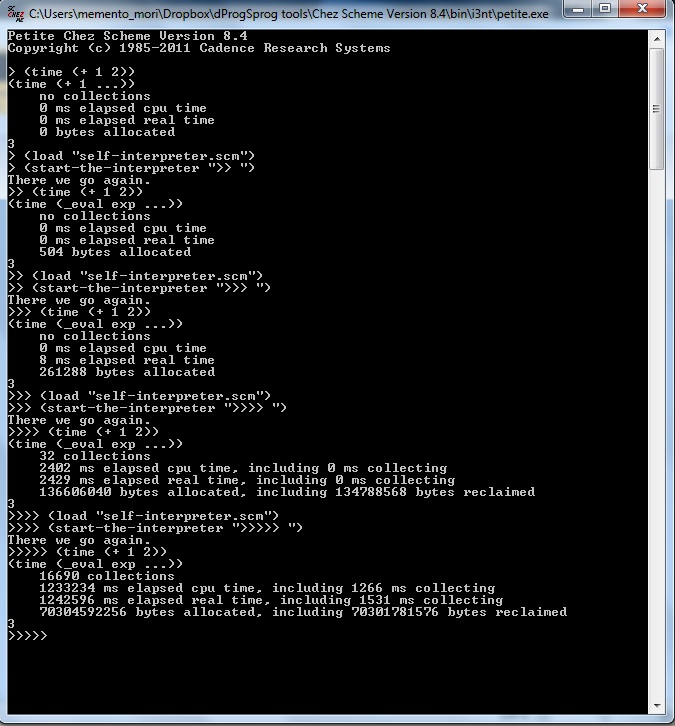
\includegraphics[width=0.75\textwidth]{HanusResults}
\end{figure}

\begin{figure}[h!]
  \caption{3 interpreters running on top of each other}
  \centering
    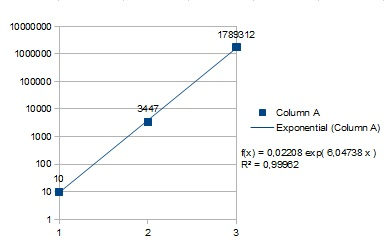
\includegraphics[width=0.75\textwidth]{HanusGraf3}
\end{figure}

\begin{figure}[h!]
  \caption{Graph with one more interpreter}
  \centering
    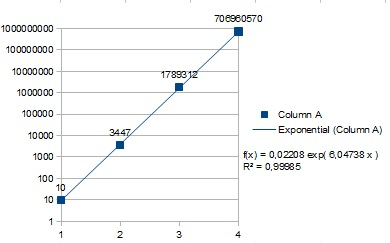
\includegraphics[width=0.75\textwidth]{HanusGraf4}
\end{figure}

\begin{figure}[h!]
  \caption{Graph with the 3 interpreters running on top of each other (on a Mac)}
  \centering
    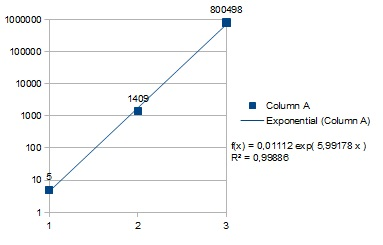
\includegraphics[width=0.75\textwidth]{AndersGraf3}
\end{figure}

\begin{figure}[h!]
  \caption{Graph with one more interpreter (on a Mac)}
  \centering
    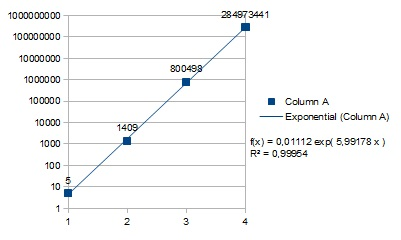
\includegraphics[width=0.75\textwidth]{AndersGraf4}
\end{figure}

\begin{figure}[h!]
  \caption{Bytes allocated result with the 3 interpreters running on top of each other}
  \centering
    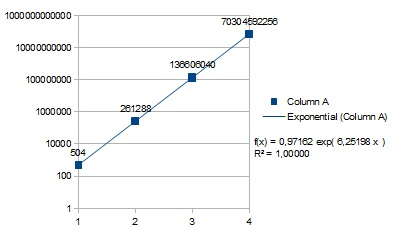
\includegraphics[width=0.75\textwidth]{HanusGrafBytesAllocatet3}
\end{figure}

\begin{figure}[h!]
  \caption{Bytes allocated result of graph with one more interpreter (4)}
  \centering
    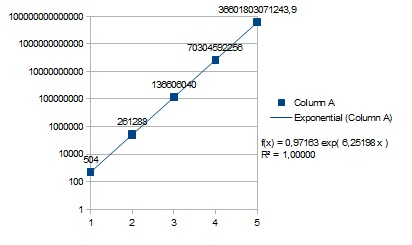
\includegraphics[width=0.75\textwidth]{HanusGrafBytesAllocatet4}
\end{figure}
\end{document}
